\documentclass[./00PhotoBox.tex]{subfiles}
\graphicspath{{\subfix{./img/}}}
\begin{document}


\chapter{Systemkalibrierung}
\label{ch:kalibrierung}

Für die Berechnung von 3D-Modellen mit korrekter Skalierung sind einige Parameter zu bestimmen. Neben der Bestimmung der inneren Orientierung der Kameras ist auch eine Realisierung eines Maßstabes notwendig. Auf die notwendigen Schritte und die möglichen Fehlerquellen wird in diesem Kapitel eingegangen.

\begin{comment}
\item Kameramodellierung
\item Kamerakalibrierung
\item Kameraausrichtung
\end{comment}

\section{Maßstab und Passpunkte}
\label{sec:passpunkt_bestimmung}
Zur Bestimmung der Skalierung (vergleiche \autoref{sec:massstab}) wurde sich für eine Kombination aus Maß\-stäben und Passpunktkoordinaten entschieden. Die Möglichkeit der festen und bekannten äußeren Orientierung der Kameras entfiel, da diese projektabhängig bewegt werden sollen.

Die Passpunkte in Form von ArUco-Markern wurden fest am Rahmen montiert. Diese sollen später als dauerhafte Realisierung des Maßstabes dienen. Außerdem wurden kalibrierte Maßstäbe im Objektraum verteilt, welche für die erstmalige Bestimmung der Passpunktkoordinaten den Maßstab bilden. Zur Unterstützung der Bildverknüpfung wurden weitere Punkte in Form von Schneider-Markern im Bildbereich verteilt (ähnlich dem Aufbau in \autoref{img:drehteller_moai}). Anschließend wurden Bilder vom gesamten System mit  einer externen Kamera mit festen Einstellungen aufgenommen. Diese Bilder wurden dann in Agisoft Metashape verarbeitet und Koordinaten der Passpunkte bestimmt. Über manuell in Agisoft bestimmte Punkte am Boden des Systems wurde das System so transformiert, dass der Boden die XY-Ebene darstellt.

\section{Kamerakalibrierung}
Die verwendeten Kameras weisen keine stabile \gls{innereOrientierung} auf. Daher ist eine Kalibrierung in Form von festen Parametern nicht möglich. Es wurde die Annahme verfolgt, dass die \gls{innereOrientierung} linear von der Fokussierung abhängig ist. Daraus wurde eine Formel zur Bestimmung von Näherungswerten für die \gls{innereOrientierung} in Abhängigkeit der Fokussierung ermittelt.

Die eigentliche Bestimmung der inneren Orientierung erfolgt im Betrieb in Form einer Simultankalibrierung (vgl. \autoref{s:innereorientierung}). Die Näherungswerte sollen dabei als Startwerte dienen.

\paragraph{Vorgehen}

Es wurden mit fünf verschiedenen Fokussierungen mit jeweils 24 Rasp\-berry-Pi-Kameras Bilder aufgenommen und die Bilder in Agisoft Metashape mittels ArUco-Markern orientiert, dessen Position aus \autoref{sec:passpunkt_bestimmung} bekannt ist. Außerdem wurden etwa 100 Schneider-Marker im Bildbereich der Kameras verteilt und als Verknüpfungspunkte benutzt. Es wurden jeweils in Metashape alle Bilder mit der gleichen Fokussierung als eine Kamera angenommen und die \gls{innereOrientierung} bestimmt. Anschließend wurden alle Kameras nochmal einzeln ausgeglichen. Dieses zweistufige Vorgehen bewirkt, dass die Näherungswerte schrittweise verbessert werden. Ein einstufiges Vorgehen ohne Näherungswerte führte zu falschen Werten. Die \gls{innereOrientierung} (vgl. \autoref{s:innereorientierung}) wurde in Form von Brennweite, \Gls{Bildhauptpunkt}verschiebung und \Gls{Verzeichnung} ermittelt und die Ergebnisse wurden in einem Box-Whisker-Plot dargestellt und eine ausgleichende Gerade ermittelt.

\paragraph{Ergebnis}

Die Ergebnisse sind in \autoref{img:naeherungswerte} dargestellt. Wie auch schon in der Voruntersuchung in \autoref{sec:fokus} zeigt sich, dass die \Gls{Kamerakonstante} $c$ linear zur Fokussierung ist. Bei der \Gls{Bildhauptpunkt}verschiebung $x'_0, y'_0$ und der radial-symmetrischen \Gls{Verzeichnung} $k_1,k_2,k_3$ ist die Abhängigkeit nicht eindeutig. \autoref{tab:naeherungswerte_corr} zeigt die Korrelationsmatrix der Näherungswerte. Die Fokussierung und die \Gls{Kamerakonstante} sind stark korreliert. Die Korrelation der \Gls{Bildhauptpunkt}verschiebung ist nur schwach, die der \Gls{Verzeichnung} nicht vorhanden. Es zeigt sich, dass die \gls{innereOrientierung} durch die Fokussierung beeinflusst wird. Die \Gls{Brennweite} ist dabei erwartungsgemäß am stärksten betroffen.

\begin{figure}
    \centering
    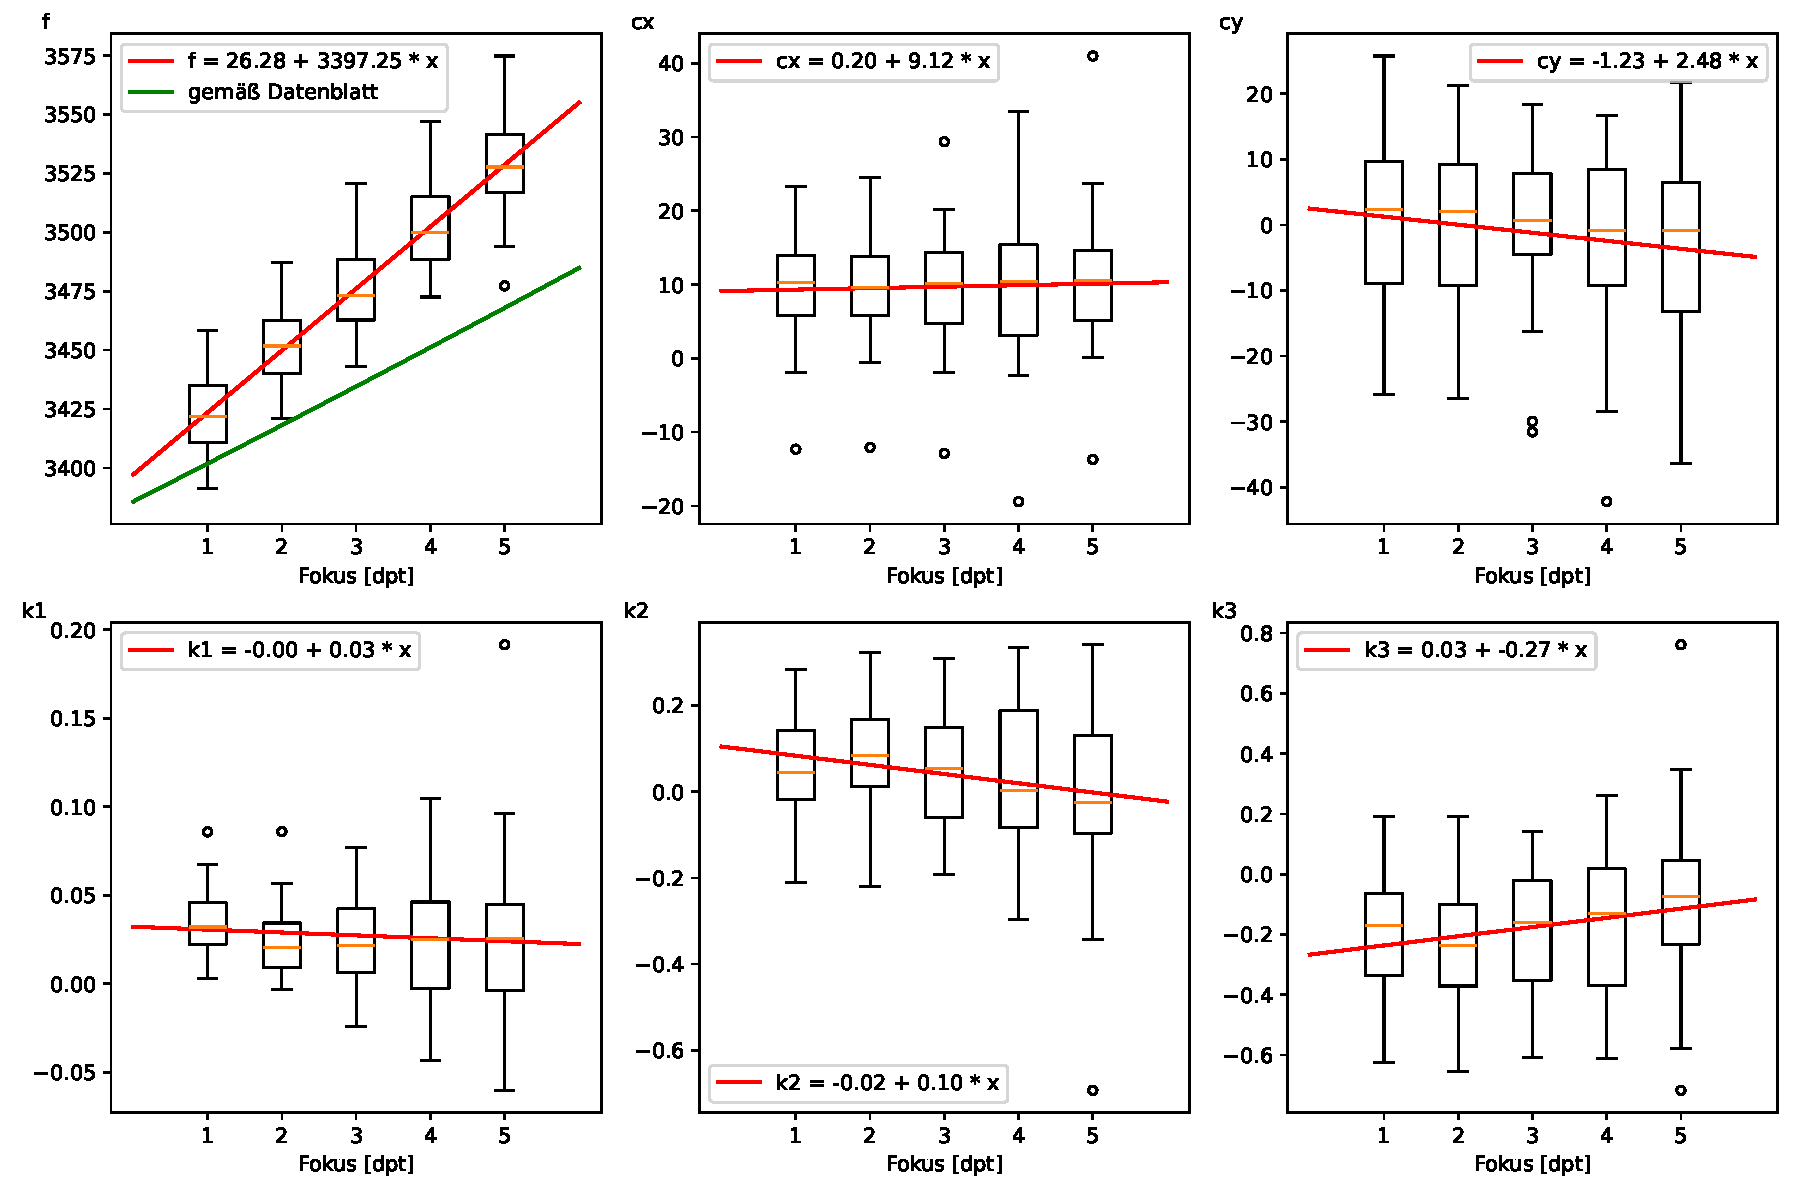
\includegraphics[width=1\textwidth]{./img/naeherungswerte_diagramm.pdf}
    \caption{Box-Whisker-Plots und ausgleichende Gerade der inneren Orientierung in Abhängigkeit von der Fokussierung [\glsentryshort{dpt}]} %Bildunterschrift
    \label{img:naeherungswerte} %ID fürs Bild
\end{figure}

\begin{table}
\caption{Korrelationsmatrix der Näherungswerte}
\label{tab:naeherungswerte_corr}
\begin{tabular}{lrrrrrrr}
\toprule
 & Fokus [dpt] & f & cx & cy & k1 & k2 & k3 \\
\midrule
Fokus [dpt] & 1,000 & 0,901 & 0,032 & -0,128 & -0,069 & -0,181 & 0,177 \\
f &   & 1,000 & -0,010 & -0,211 & -0,220 & -0,071 & 0,092 \\
cx &   &   & 1,000 & -0,230 & 0,005 & 0,005 & 0,005 \\
cy &   &   &   & 1,000 & 0,031 & 0,023 & -0,051 \\
k1 &   &   &   &   & 1,000 & -0,925 & 0,866 \\
k2 &   &   &   &   &   & 1,000 & -0,985 \\
k3 &   &   &   &   &   &   & 1,000 \\
\bottomrule
\end{tabular}
\end{table}


\begin{comment}
\section{Farbkalibrierung}

Für die korrekte Texturierung des 3D-Modelles sollte die Farbe möglichst korrekt sein. Da das System aber nicht von Fremdlichtquellen abgeschirmt ist, soll dies nur verhindern, dass die Farbe schon ohne Fremdlicht falsch sind. Daher wurde mit dem System eine Farbkalibriertafel fotografiert und die Farbwerte ausgewertet. Hiermit lassen sich dann die Farben der Kameras korrigieren. \citep[S. 431f]{luhmann}
\end{comment}

\biblio
\end{document}